\chapter{Facility Description}
\label{vl:tc-facility}


%\section{Detector Caverns Cryostats and Cryogenics}
%\label{sec:fdsp-coord-faci-caverns}


The underground facilities for the \dword{dune} detectors have two parallel
detector caverns with one central utility cavern between them. The
long direction of the caverns aligns approximately
east/west. Therefore, the two detector caverns are called the north
and south caverns. Figure~\ref{fig:dune-underground} shows the overall
underground campus at the \dword{surf} 4850 level. Note that the bottom of the cryostats are at the 4910 level.
\begin{dunefigure}[Underground campus]{fig:dune-underground}
  {Underground campus at the 4850 level.}
  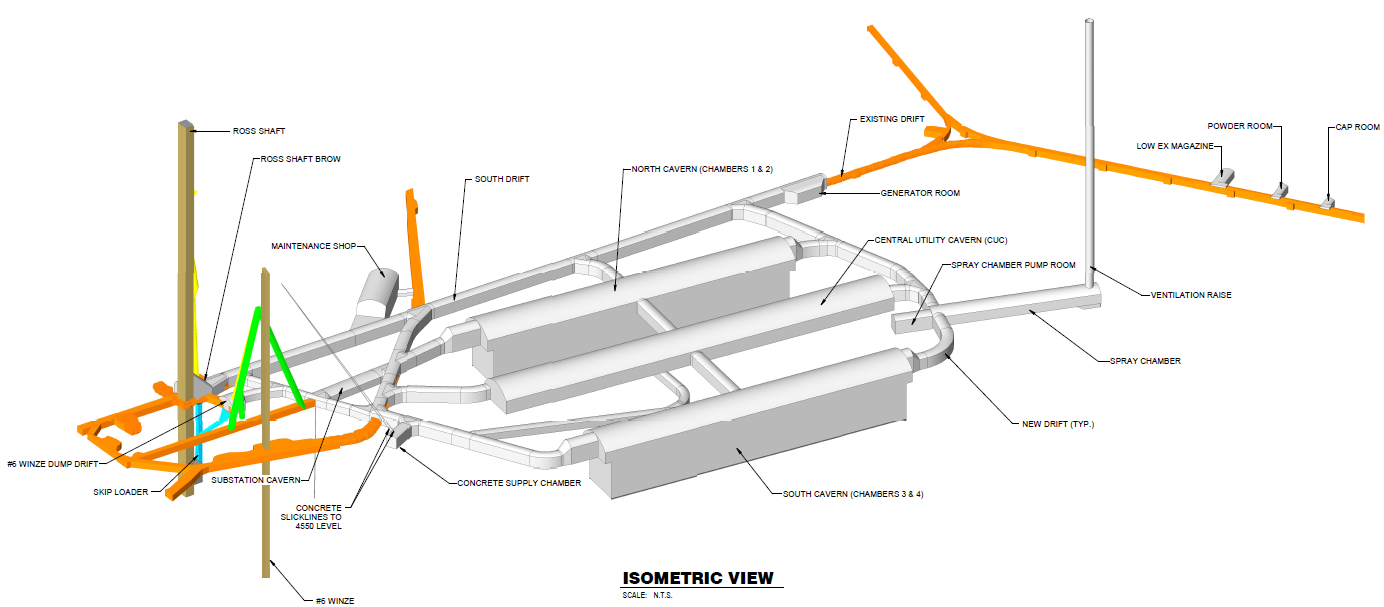
\includegraphics[width=0.85\textwidth]{Underground_campus.png}
\end{dunefigure}
Each detector cavern is \SI{144.5}{\meter} long, \SI{19.8}{\meter}
wide and \SI{27.95}{\meter} high, with one detector on the west side
and one on the east side. Between the two detector modules in one
cavern is a \SI{12}{\meter} space for detector access, cryogenic pumps and
a temporary clean
room for installing the detectors. Access tunnels lie at the east and
west ends of each cavern, north and south side of north cavern and
north side of south cavern.


The \dword{cuc} is \SI{190}{\meter} long, \SI{19.3}{\meter}
wide, and \SI{10.95}{\meter} high; it will house cryogenic equipment, \dword{daq}
room and mechanical and electrical services for all four
detectors.


Each detector is housed inside a cryostat. Each cryostat is made of
(from outside to inside): external steel structure, warm membrane
plate, insulation and cold membrane. Figure~\ref{fig:dune-cryostat}
shows the overall construction. The cryostat will have a vertical
\dword{tco} at one end to allow installation of detector components. The
opening will be closed after the majority of detector installation is
complete and before filling. After the \dword{tco} closing the last of the
detector installation will be completed. After final detector
installation and equipment removal through the roof openings, the
cryostat will be closed for purge, cooldown and filling.
\begin{dunefigure}[\dword{dune} cryostat]{fig:dune-cryostat}
  {Overall construction and dimensions of the \dword{dune} cryostat.}
  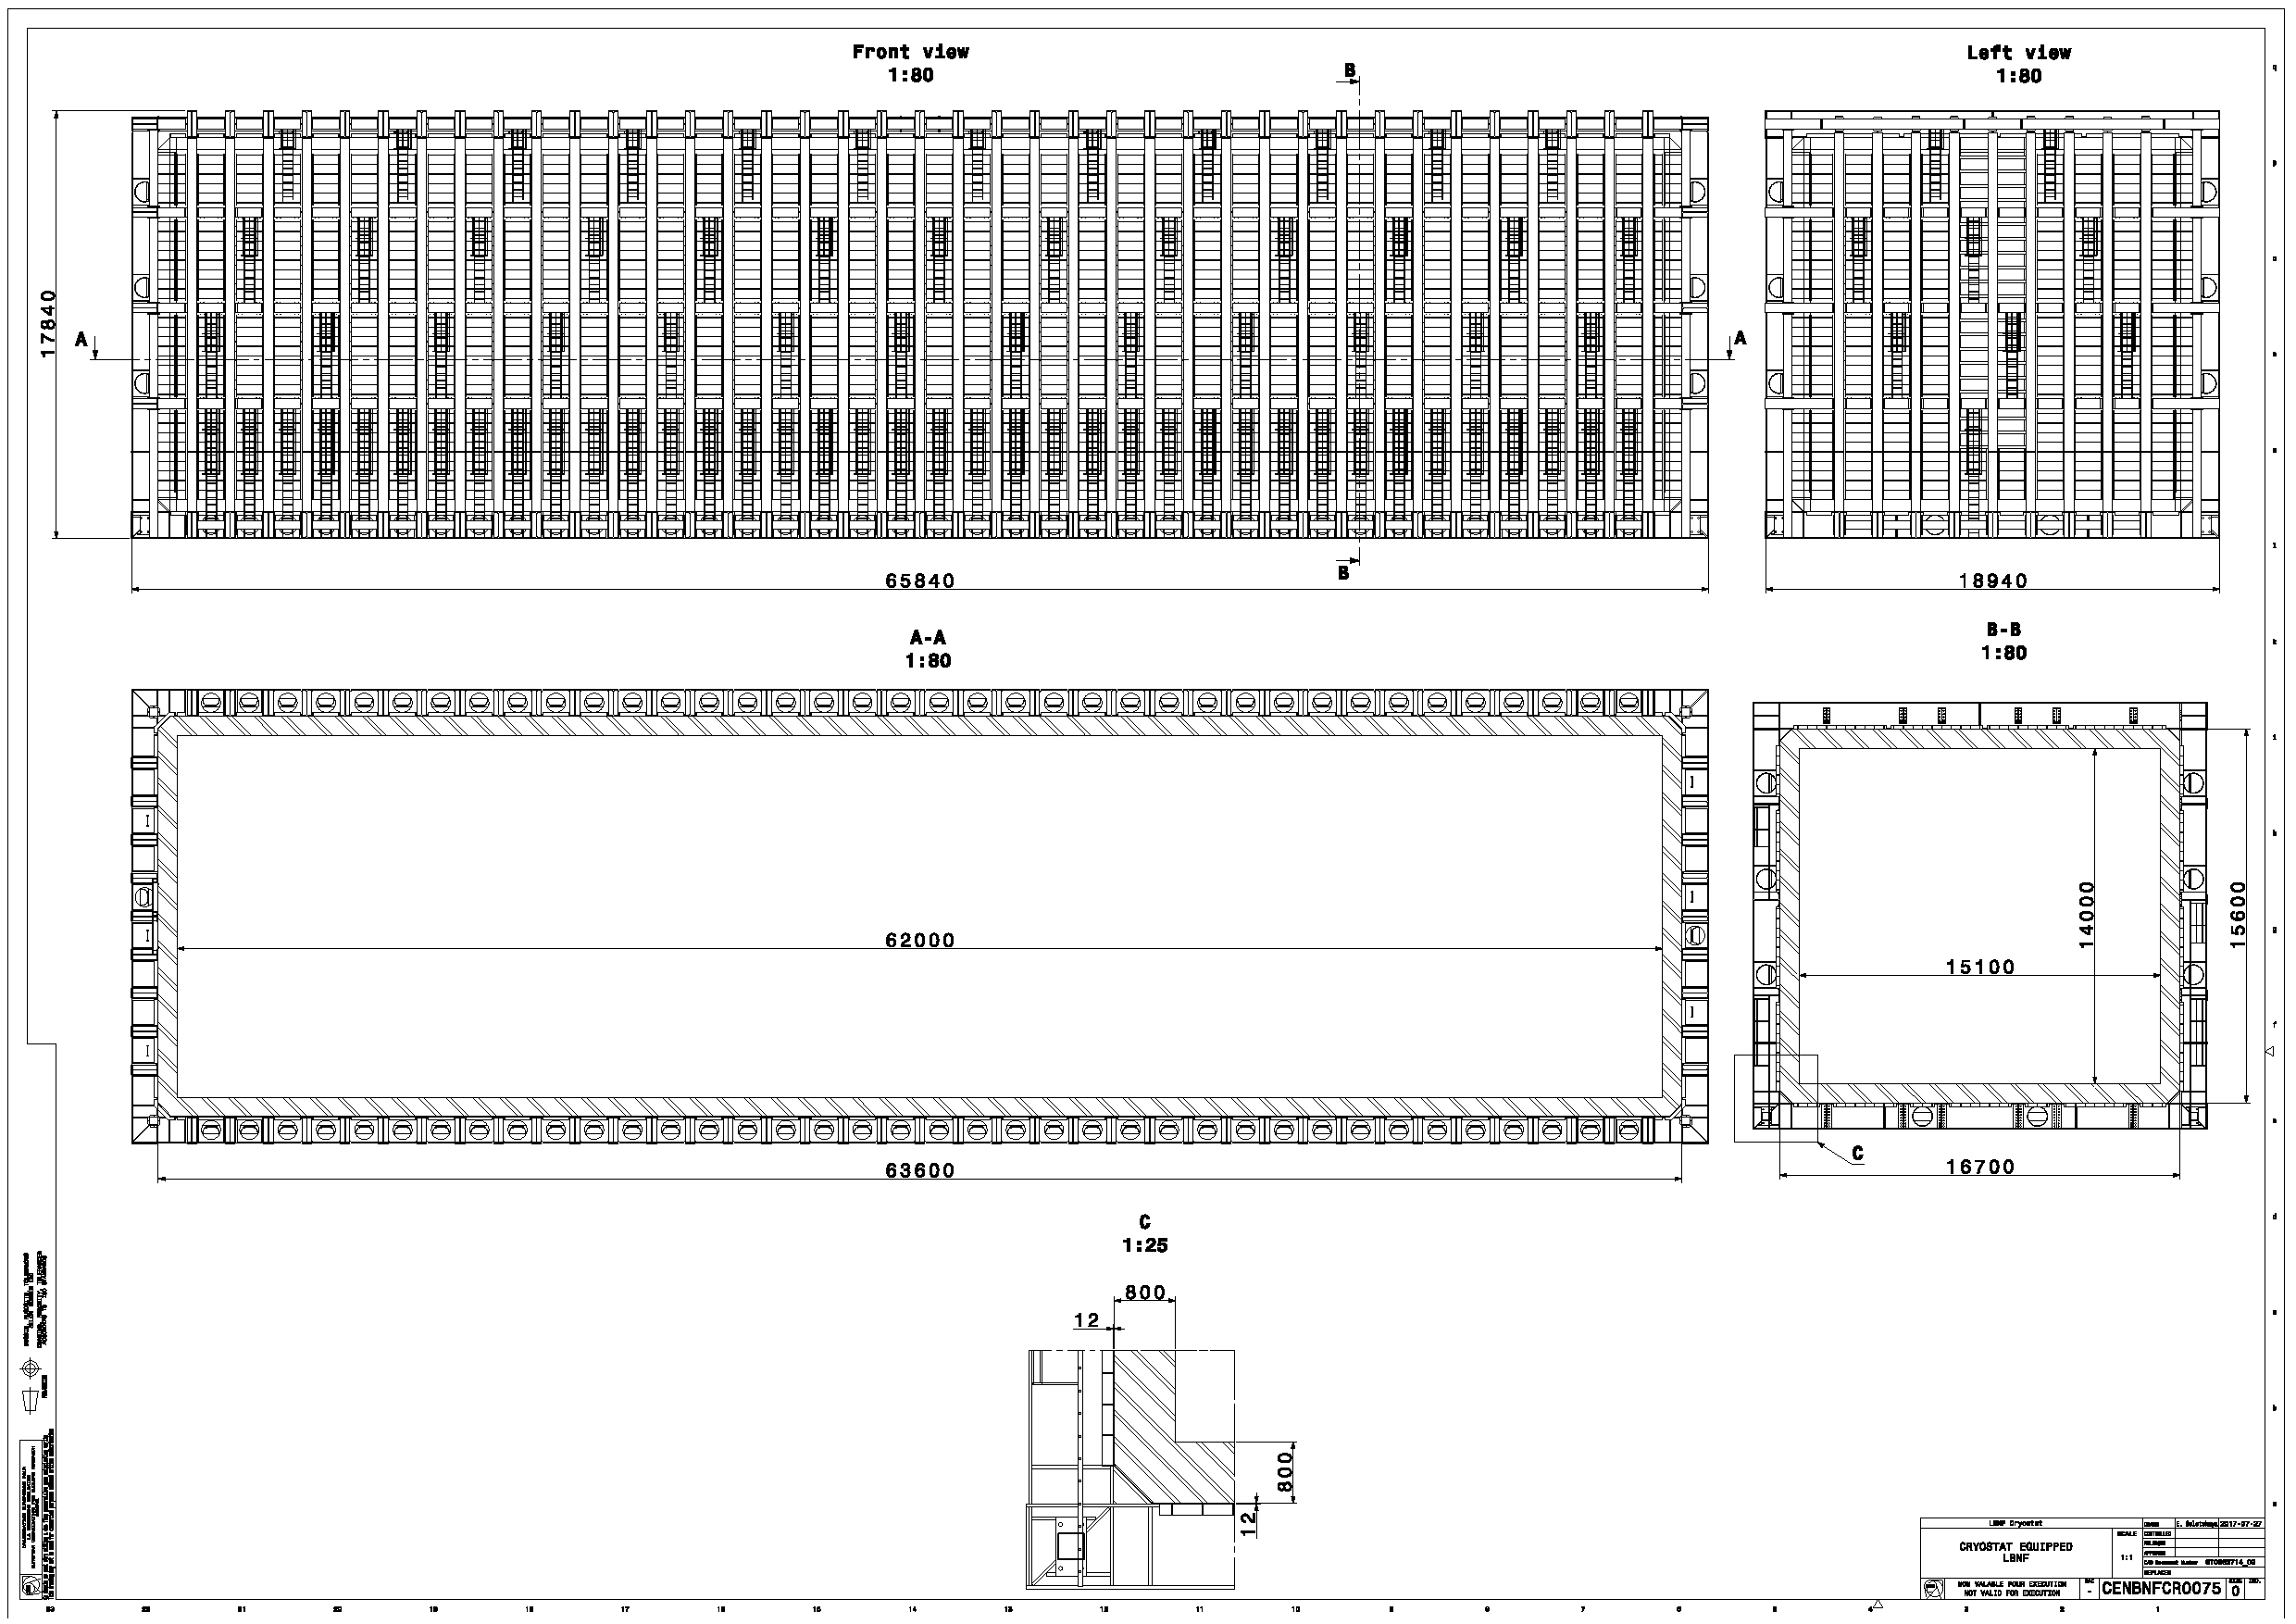
\includegraphics[width=0.85\textwidth]{cryostat.pdf}
\end{dunefigure}


The detector cryogenics system supplies \dword{lar} and provides
circulation, re-condensation and purification. The cryogenic system
components are housed inside the \dword{cuc}, on top of each detector module
and between detector modules. The cryogenic system comprises
\begin{itemize}
\item {\bf Cryogenic infrastructure}: This includes \dword{lar} and LN$_2$ receiving
  facilities on the surface, nitrogen refrigeration systems (both
  above ground and underground), LN$_2$ buffer storage
  underground, piping to interconnect equipment (LN$_2$, GN$_2$ and GAr),
  components in the detector cavern and the \dword{cuc} and process control/support
  equipment.
\item {\bf Proximity cryogenics}: This includes reliquefaction 
  and
  purification subsystems for the argon (both gas and liquid), associated
  instrumentation and monitoring equipment and \dword{lar} piping to
  interconnect equipment and components in the detector cavern and the
  \dword{cuc}. The proximity cryogenics are split into three areas: in the
  \dword{cuc}, on top of the mezzanine and on the side of the cryostat 
  where \dword{lar} circulation pumps are installed.
\item {\bf Internal cryogenics}: This includes \dword{lar} and GAr distribution
  systems inside the cryostat, as well as features to cool the
  cryostat and the detector uniformly.
\end{itemize}
Figure~\ref{fig:dune-cryogenics} shows the process flow diagram of the
\dword{lbnf} cryogenic system. Only one cryostat is shown.
\begin{dunefigure}[Cryogenics system]{fig:dune-cryogenics}
  {Overall process flow diagram of the cryogenic system showing one
    cryostat only; other cryostats are the same.}
  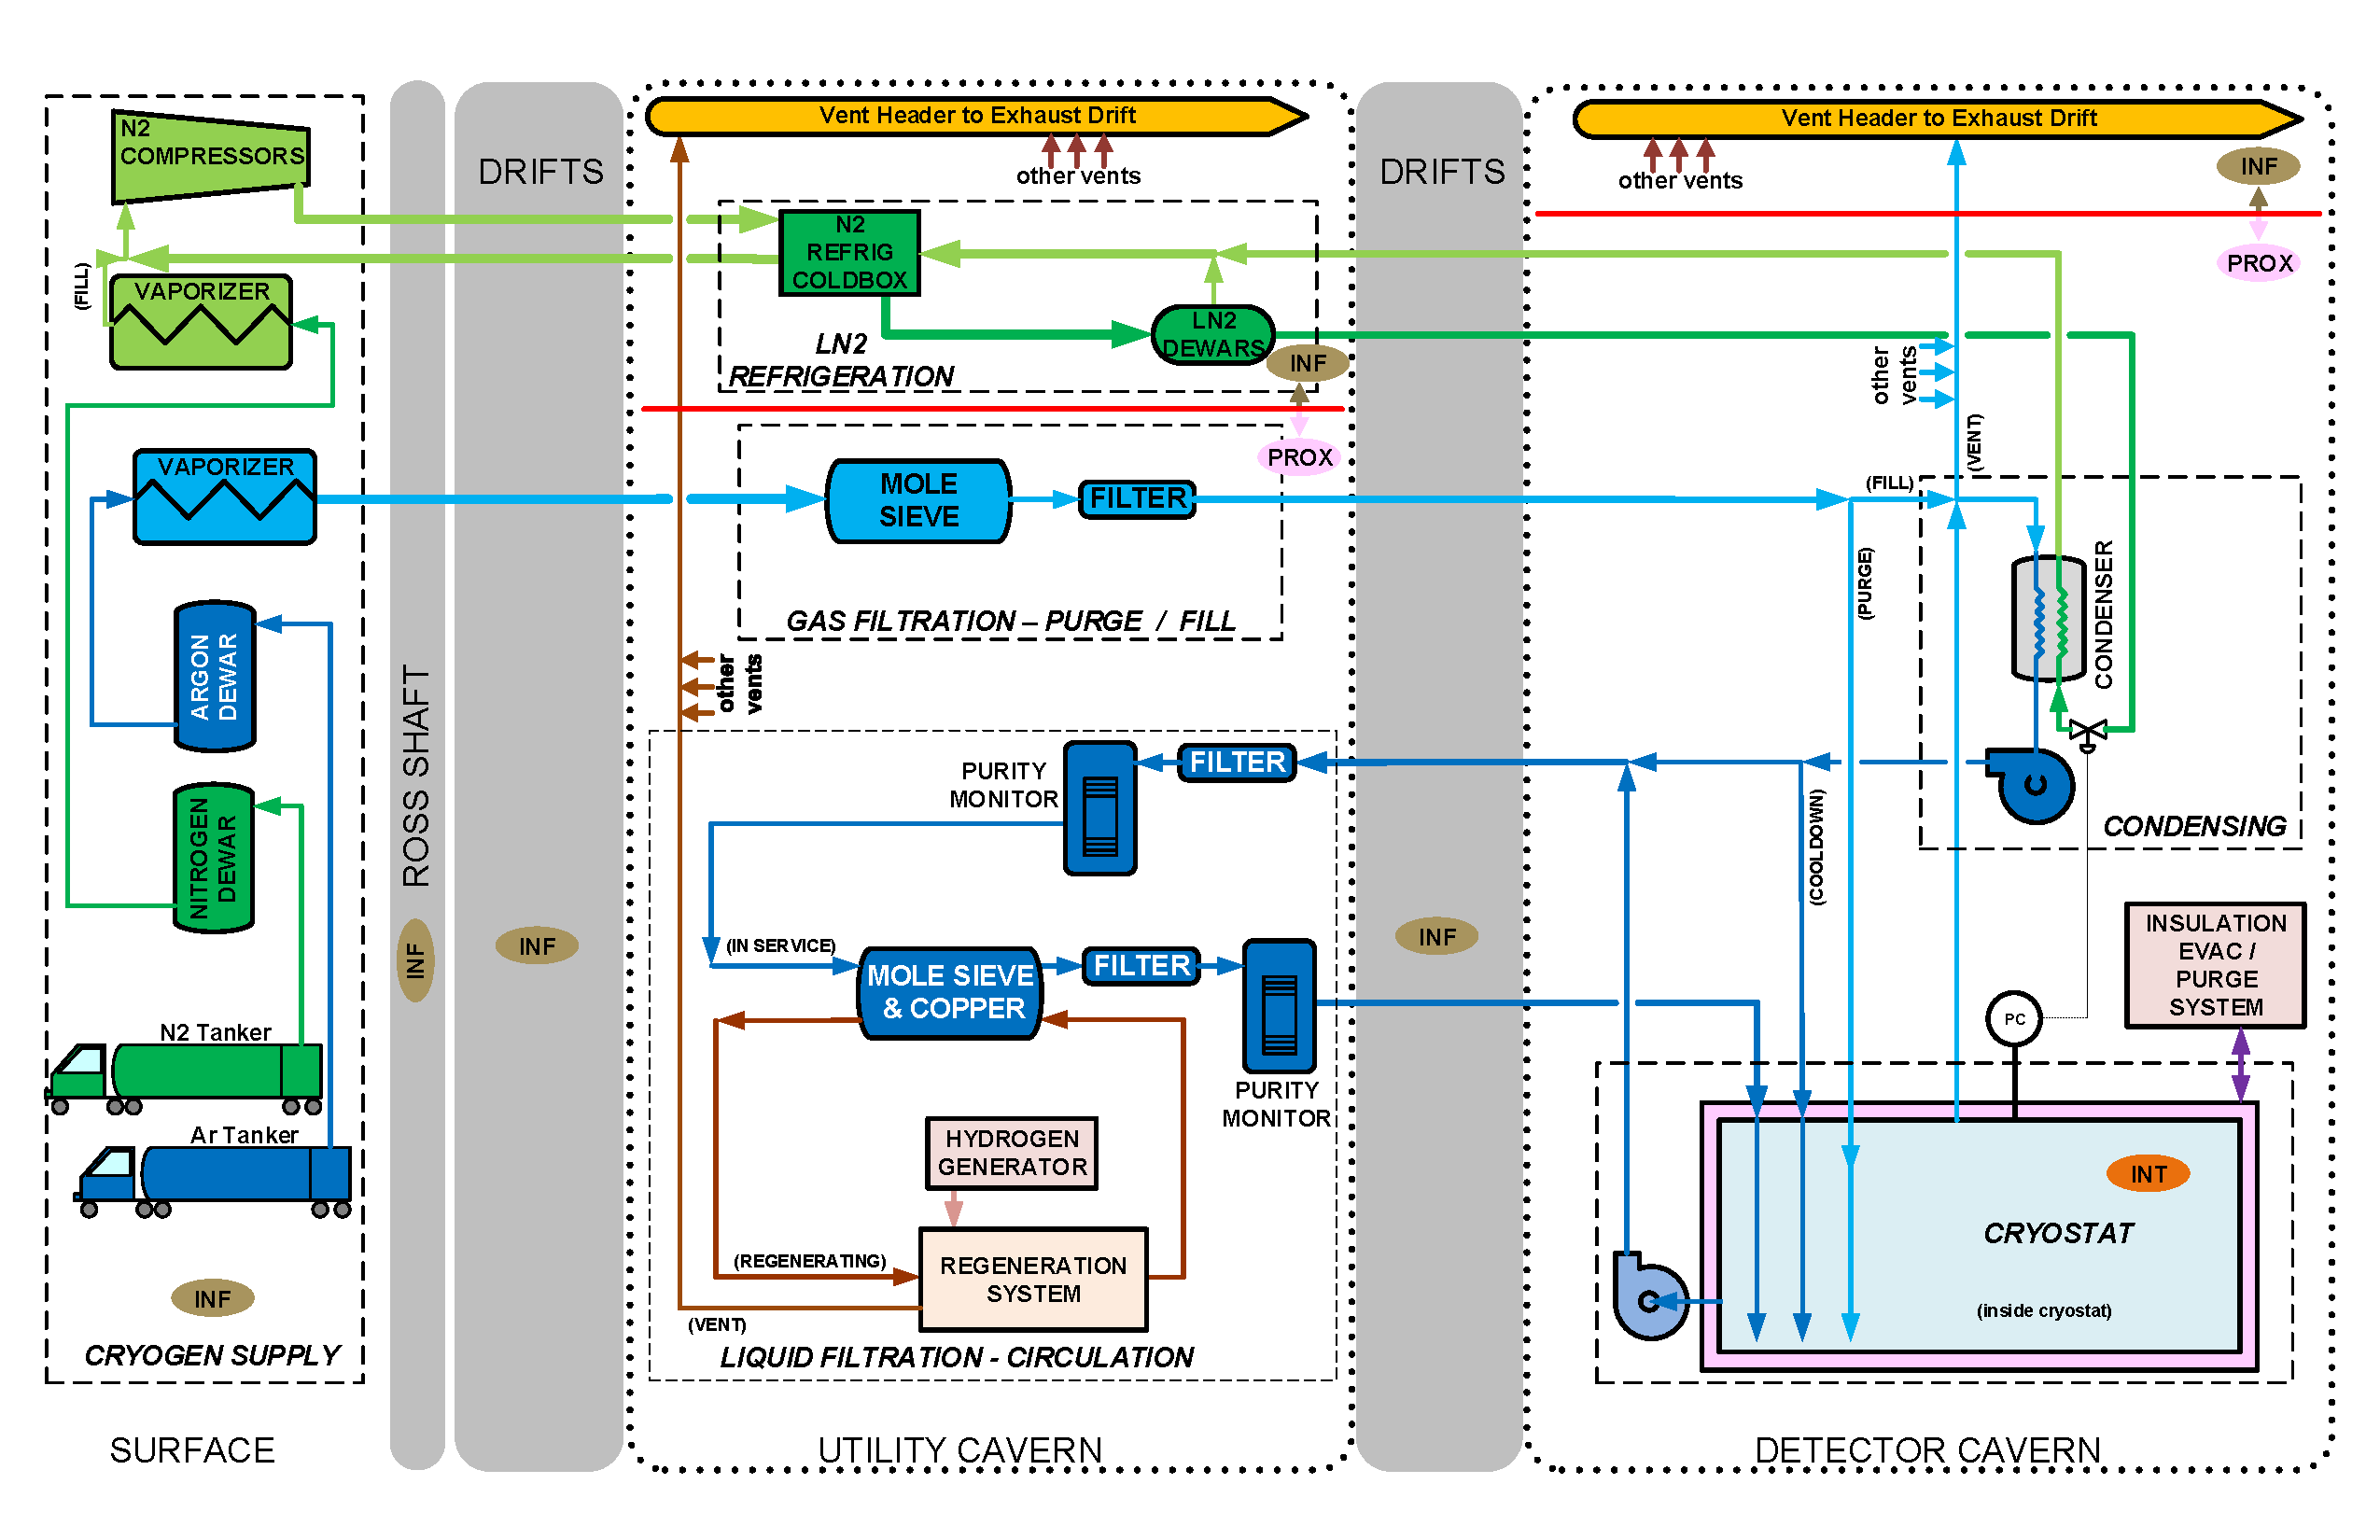
\includegraphics[width=0.85\textwidth]{LBNF_PFD_180909.pdf}
\end{dunefigure}


The underground facilities include all the \dword{bsi} and utilities,
such as HVAC systems for underground environment control, chilled
water for cooling detector electronics and cryogenics compressors,
material handling equipment (monorails and bridge cranes), industrial
water systems and lighting required for constructing and operating
detectors.


\section{Detector Grounding}
\label{sec:fdsp-coord-faci-grounding}


The detector grounding strategy provides detectors with an independent
isolated ground to minimize any environmental electrical noise that
can couple into the detector electronics either conductively or
through emitted electromagnetic interference.


The detectors will be placed at the 4910 level of \surf. The
electrical conductivity of the various rock masses are unknown but
should have extremely poor and inconsistent conductive
properties. Ensuring adequate sensitivity of the detectors requires a
special ground system that will isolate the detectors from all other
electrical systems and equipment, minimize the influence of inductive
and capacitive coupling, and eliminate ground loops. The grounding
infrastructure should reduce or eliminate ground currents through the
detector that would affect detector sensitivity, maintain a low
impedance current path for equipment short circuit and ground fault
currents, and ensure personnel safety by limiting any potential for
equipment-to-equipment and equipment-to-ground touch.


Three basic ground structures govern
construction of the caverns. Figure~\ref{fig:dune-grounding} shows these structures.
\begin{dunefigure}[Overall \dword{dune} grounding structure]{fig:dune-grounding}
  {Overall \dword{dune} grounding structure incorporated in cavern.}
  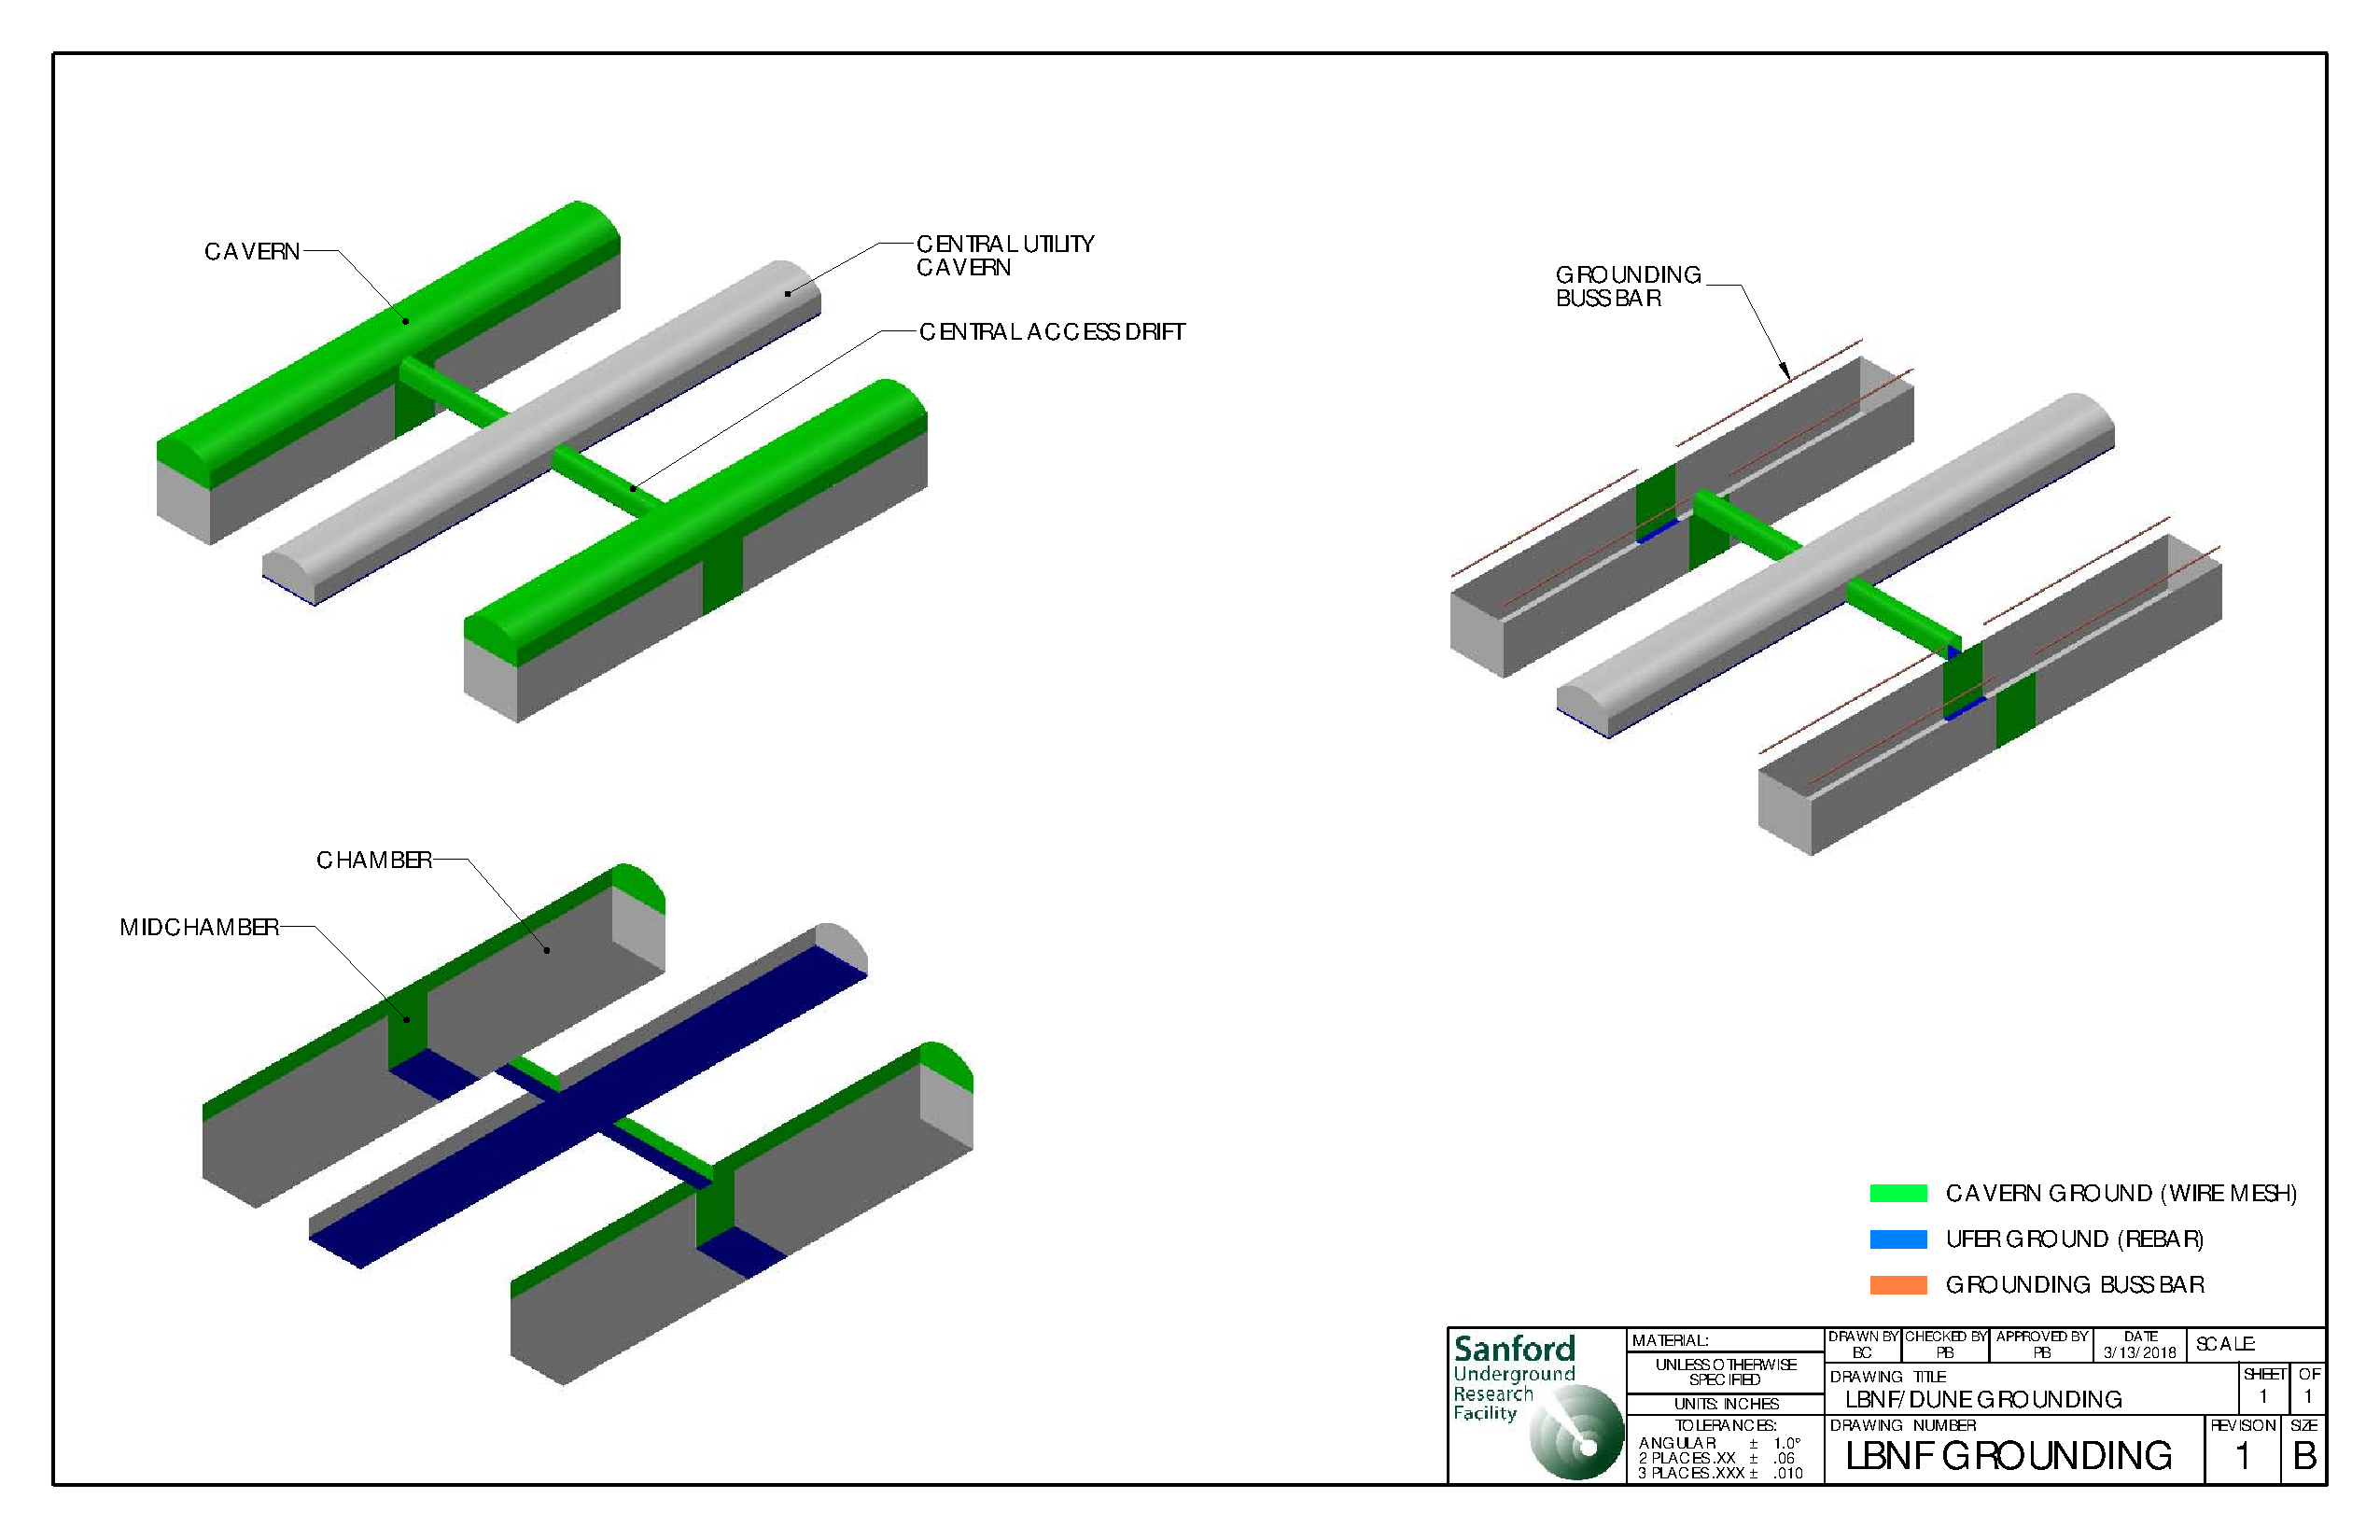
\includegraphics[width=0.85\textwidth]{SURF_Grounding.pdf}
\end{dunefigure}
These include:
\begin{enumerate}
 \item Cavern ground consisting of overlapping welded wire mesh
   supported by rock bolts and covered with shotcrete. The
   \dword{lbnf}/\dword{dune} cavern ground includes all walls and
   crown areas above the 4850 level in the north and south detector
   caverns and their associated central access drifts, as well as tin-plated
   copper bus bars that run the length of the detector vessels
   on each side along the cavern walls and are mounted external to the
   shotcrete.  The cavern ground structure
\begin{enumerate}
 \item spans the full length of the cavern from the west end access
   drift entrance through the mid-chamber to the east end access drift
   entrance;
 \item spans the full width of the cavern from the 4850 level sill
   (top of the detector vessels and mid-chamber floor) on both sides
   up and across the crown of the cavern;
 \item includes mid chamber walls to the 4910 level;
 \item includes the east and west end walls of the cavern, from the
   4850 level to the crown.
\end{enumerate}
 \item \dword{ufer} ground consisting of metal rebar embedded in
   concrete floors. The \dword{lbnf}/\dword{dune} \dword{ufer} ground
   system includes the concrete floors in the cavern mid-chambers,
   center access drifts, and central utility cavern. The cavern and
   \dword{ufer} grounds will be well bonded electrically to construct
   a single facilities ground isolated from detector ground.
 \item Detector ground consists of the steel containment vessel
   enclosing the cryostat and all metal structures attached to or
   supported by the detector vessel.
\end{enumerate}


To ensure safety, a safety ground with one or more saturated inductors
will be installed between the detector ground and the electrically
bonded \dword{ufer} and cavern grounds.
Figure~\ref{fig:dune-grounding_figure} shows the position of the
safety ground. These safety ground inductors saturate with flux under
low-frequency high currents and present minimal impedance to that
current.  Thus, an AC power fault current would be shunted to the
facility ground and provide a safe grounding design. At higher
frequencies and lower currents, such as coupled noise currents, the
inductor provides an impedance to this current, restricting its flow
between grounded metal structures. The desired total impedance between
the detector ground structure and the cavern/\dword{ufer} ground
structure should be a minimum of \SI{10}{Ohms} at \SI{10}{MHz}.
\begin{dunefigure}[Simplified detector grounding]{fig:dune-grounding_figure}
  {Simplified detector grounding scheme.}
  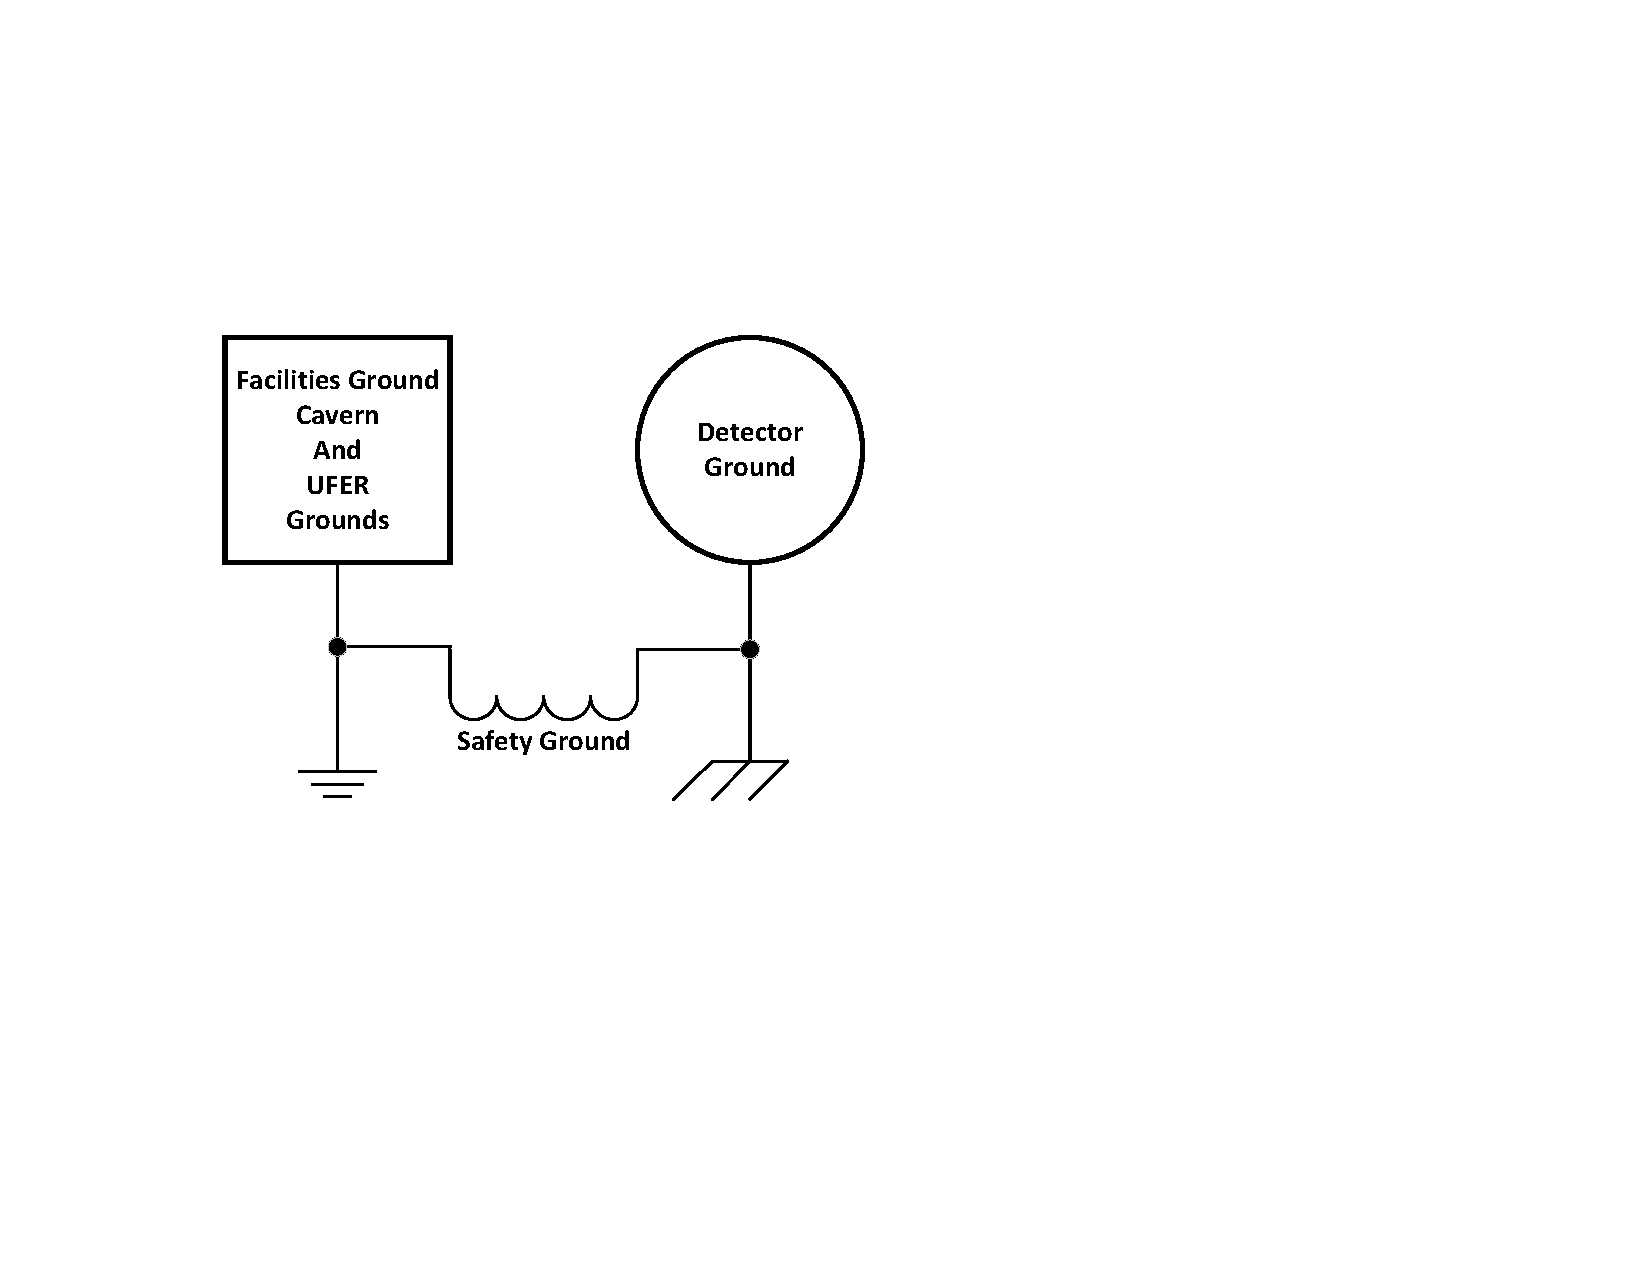
\includegraphics[width=0.5\textwidth]{Simplified_Grounding_Figure.pdf}
\end{dunefigure}


\section{Data Fibers}
\label{sec:fdsp-coord-faci-fibers}


The \dword{dune} experiment requires sixty-six fiber
optic pairs that run between the surface and the 4850 level.  A
total of 96 fiber pairs, which includes both \dword{dune} and \dword{lbnf}
needs, will be supplied through redundant paths with bundles
coming down both the Ross and Yates shafts.


The experiment requires a total of 15 data fiber pairs and one slow
control pair per detector for a total of 64.  Another two pairs are
reserved for \dword{gps}. These fibers are specified to work at
100~Gbps and meet or exceed the G.652 standard.


\section{Central Utility Cavern Control and DAQ Rooms}
\label{sec:fdsp-coord-cuc-daq}


The \dword{cuc} contains various cryogenic equipment and the \dword{daq} and control
rooms for the \dword{dune} experiment.  Both rooms are in the east
area of the \dword{cuc} (see Figure~\ref{fig:dune-cuc}).  
\begin{dunefigure}[DAQ and control rooms in CUC]{fig:dune-cuc}
  {Location of underground DAQ and control rooms in the CUC.}
  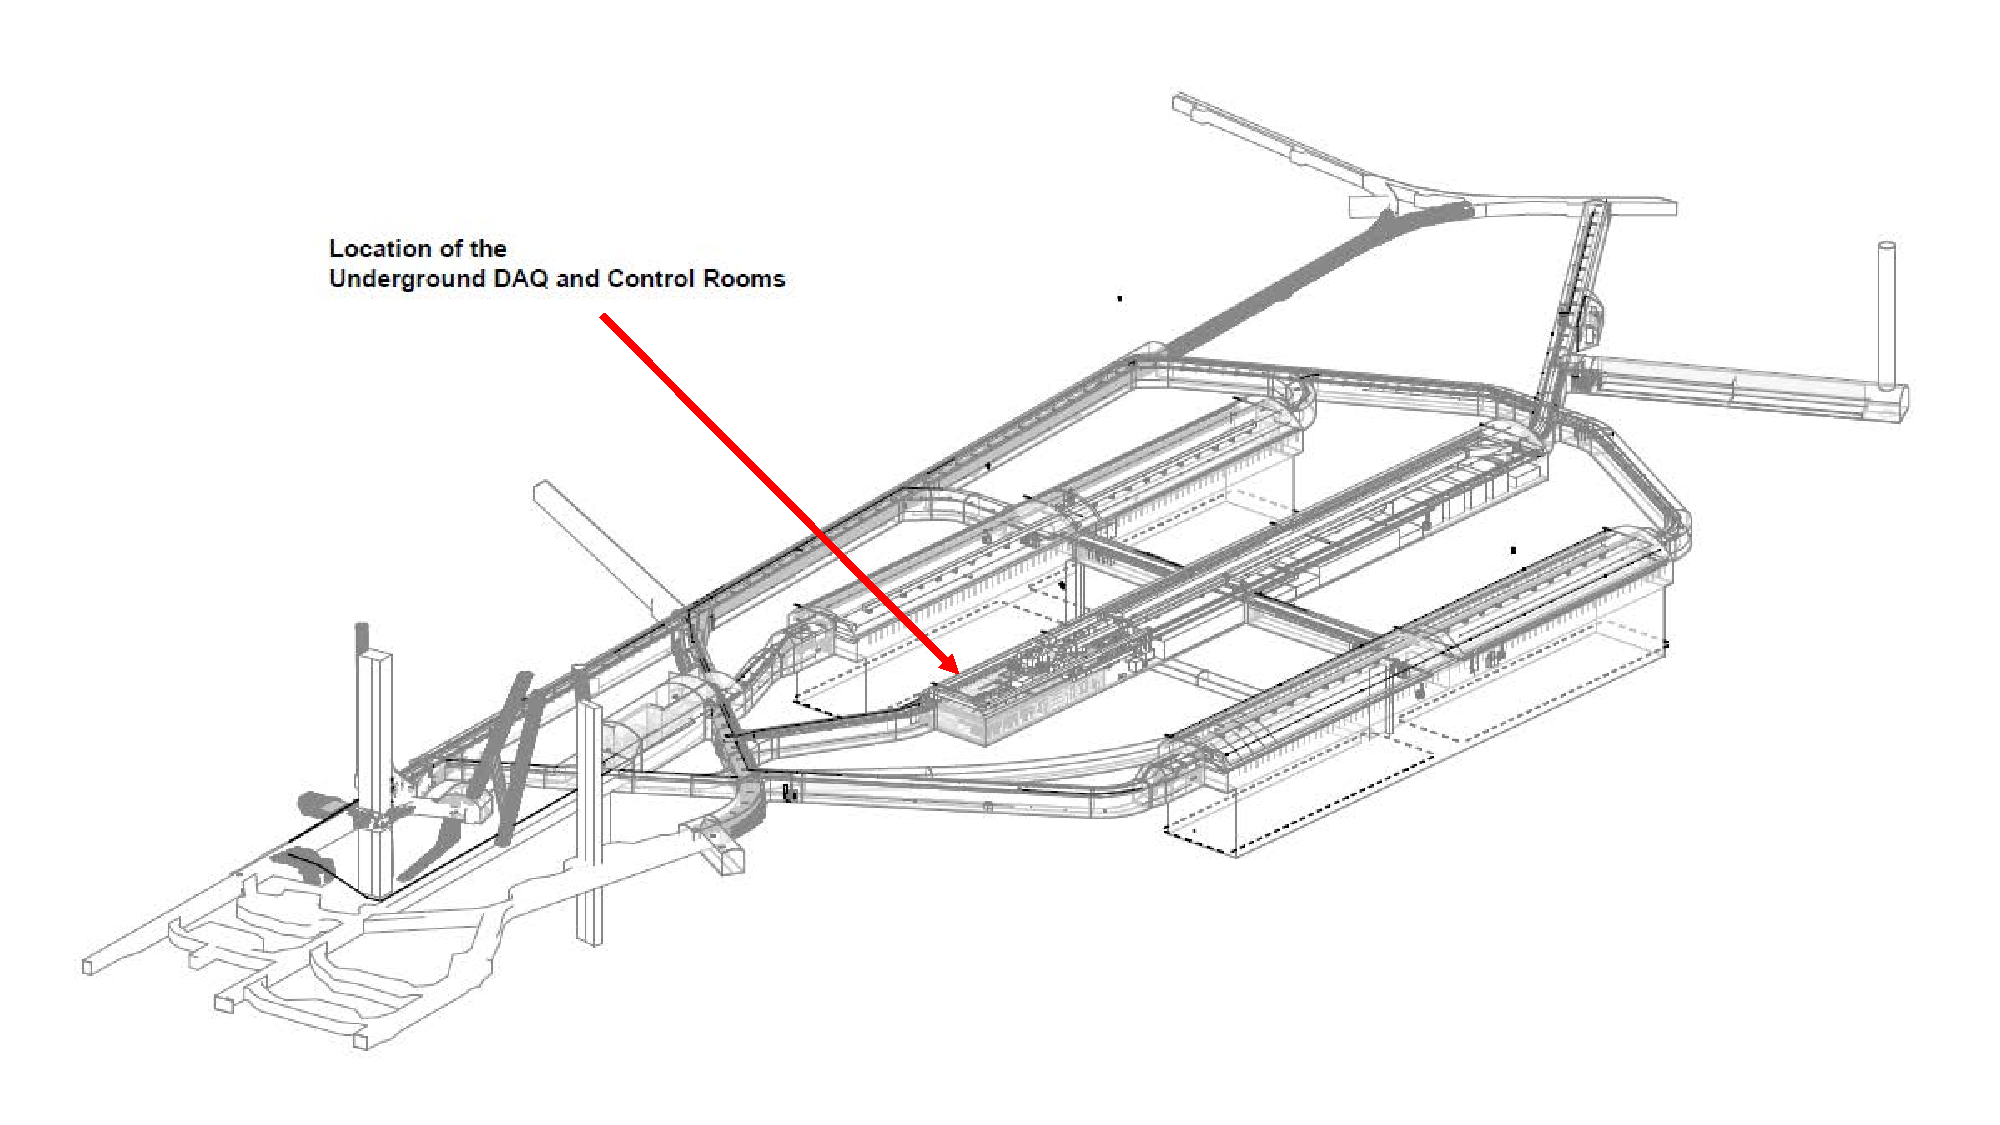
\includegraphics[width=0.85\textwidth]{Location_Underground_DAQ_Control_Rooms.pdf}
\end{dunefigure}
Figure~\ref{fig:dune-daq} shows the size and suggested outfitting of the rooms.
\begin{dunefigure}[DAQ and control rooms]{fig:dune-daq}
  {Underground DAQ and control rooms layout.}
  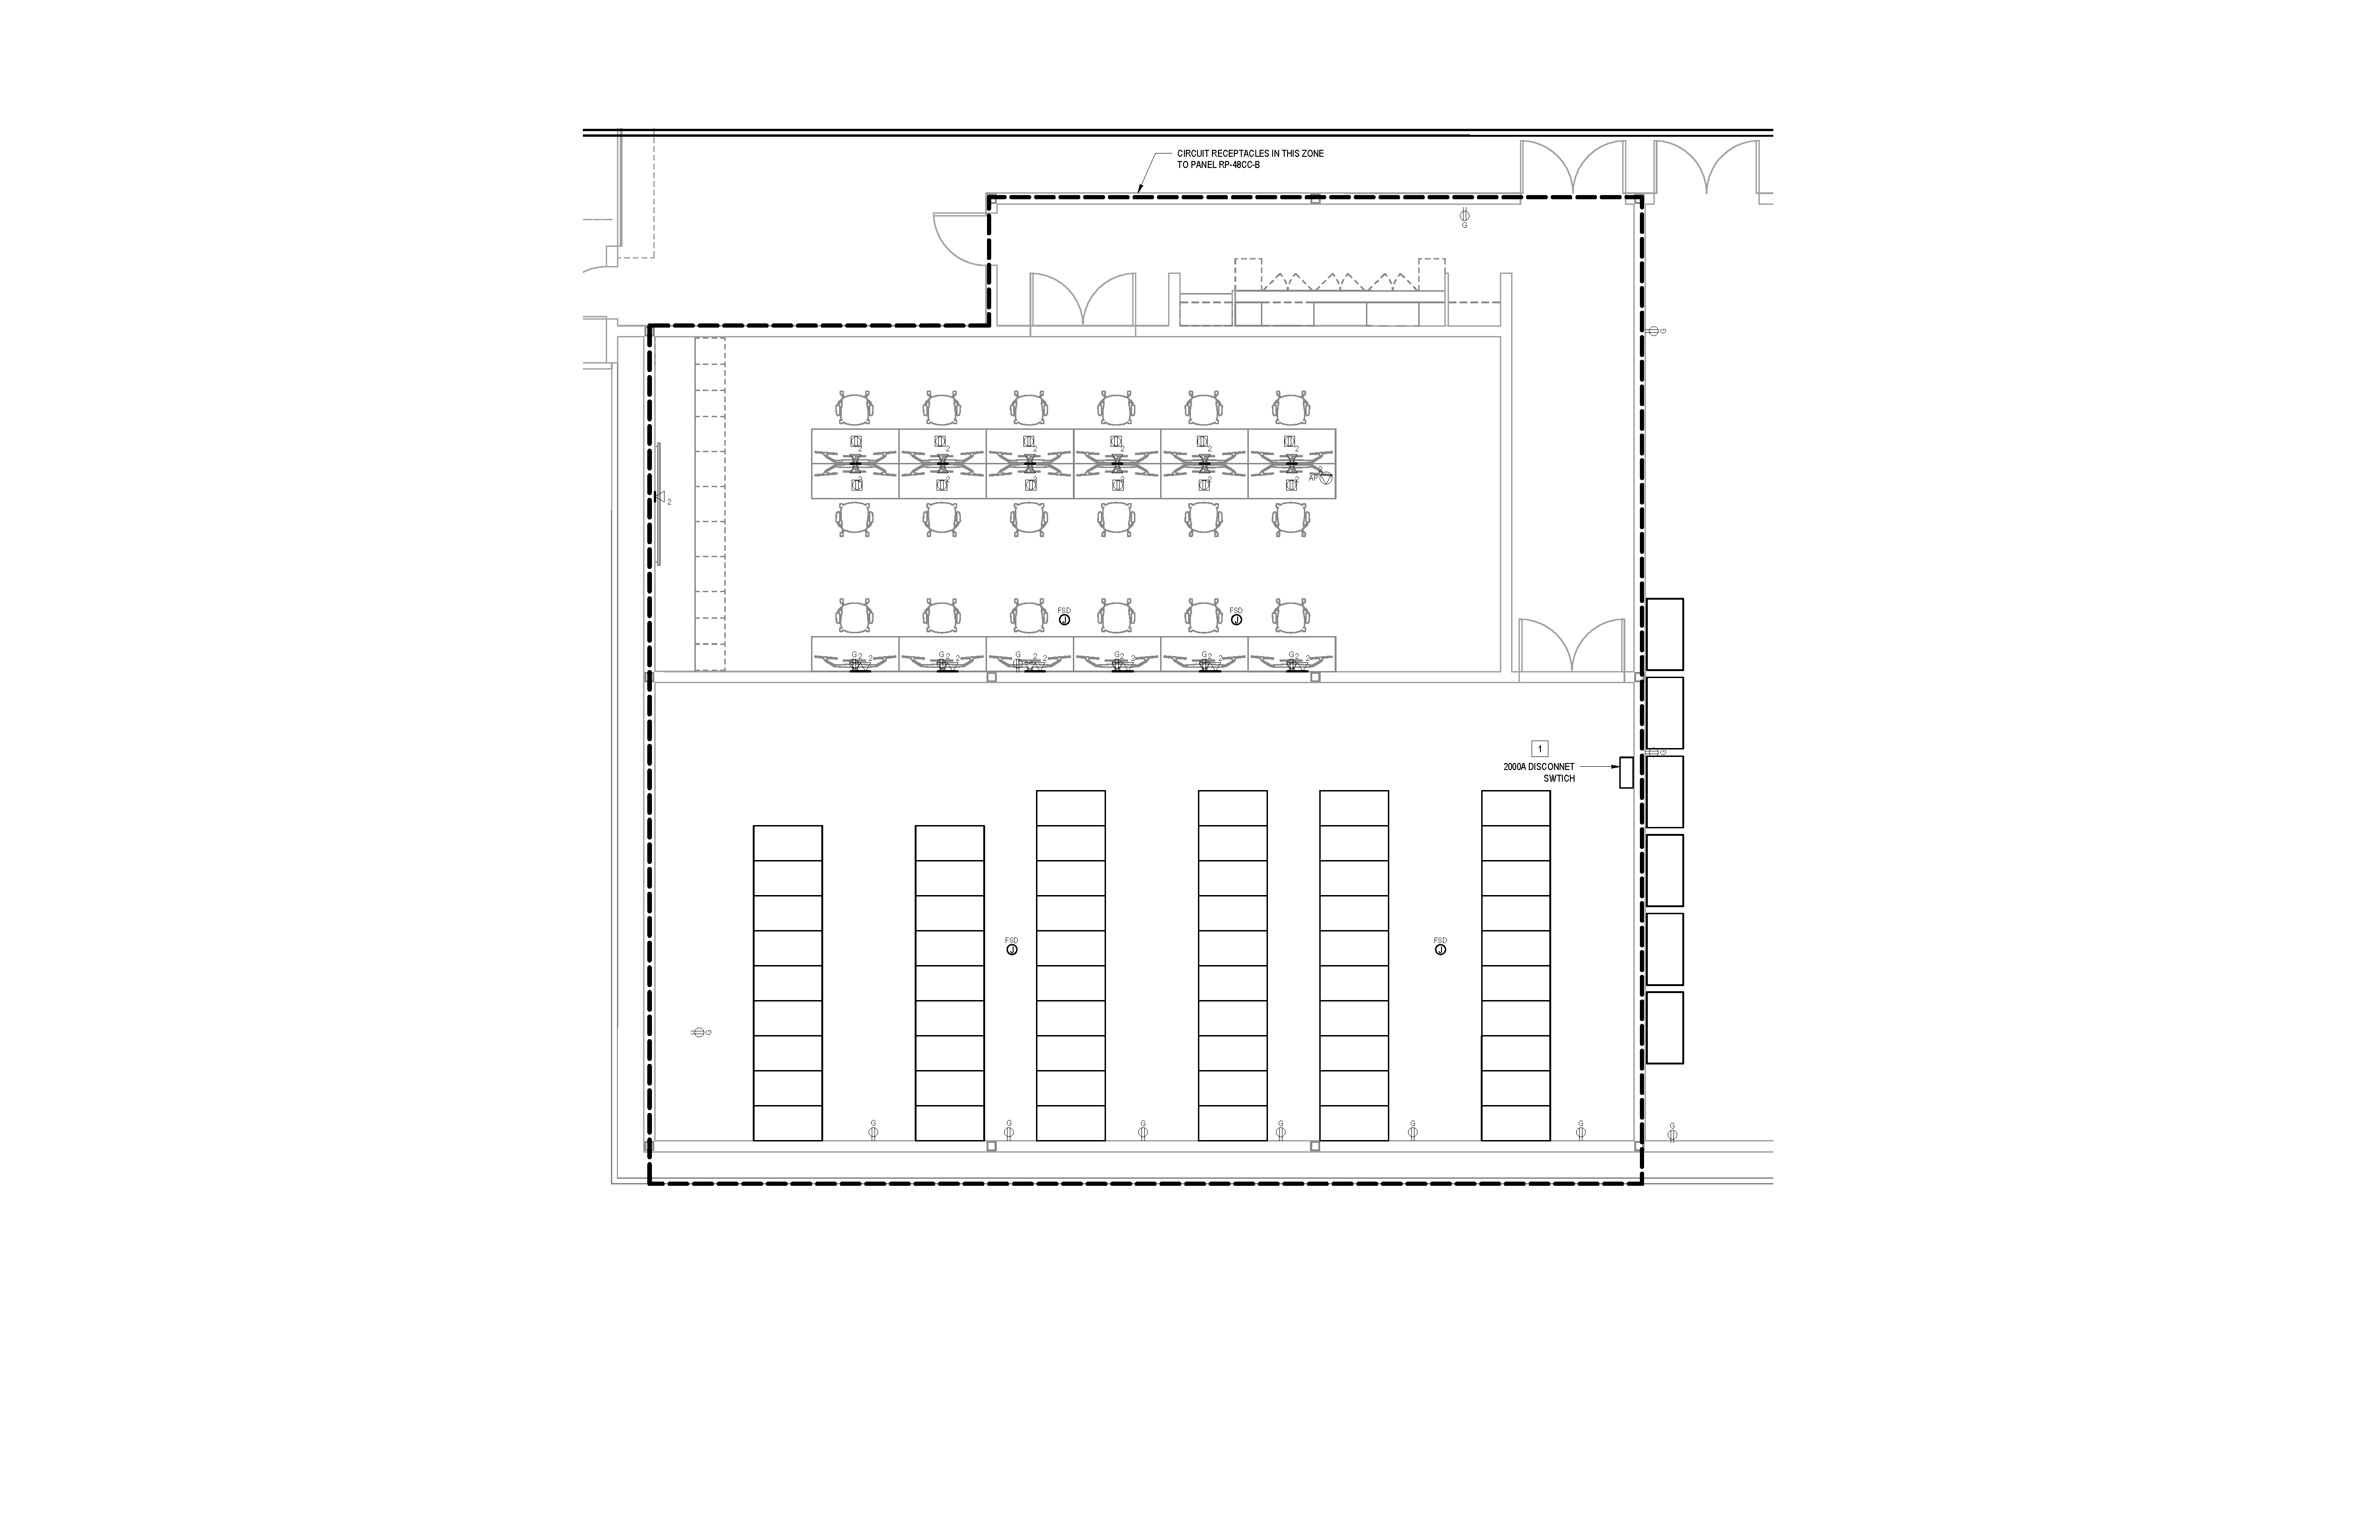
\includegraphics[width=0.5\textwidth]{Preliminary_Layout_DAQ_Control_Rooms.pdf}
\end{dunefigure}


The control room is primarily a meeting or work space where
five to ten people can sit with laptops during system commissioning.
It is not truly a control room (despite its name) from which the
experiment will be run.  The room also provides the required work space for
monitoring the cryogenic systems.  The cryogenic team requires a
footprint of two racks and two work benches for the technicians who monitor the cryogenic systems.
       
The \dword{daq} room will contain a minimum of 52 racks that will be
used for fiber optic cable distribution, networking, \dword{dune}
\dword{daq} and the requirements of conventional facilities.  A
minimum of 48 racks are reserved exclusively for \dword{daq}.
Conventional facilities supply the \dword{daq} room with cooling
water, an 18~inch raised floor, lighting, HVAC, dry fire protection
and 500kVA available power.  \Dword{tcoord} will be responsible for
the final outfitting and layout of the room.  This includes the layout
and installation of water cooled racks, design and installation of
piping that carries cooling water to the racks, the AC power
distribution to the racks and installation of cable trays.


\section{Surface Rooms}
\label{sec:fdsp-coord-surf-rooms}


The \dword{dune} experiment requires three surface rooms: surface
control room, \dword{daq} surface computer room and  facilities room.


The \dword{dune} surface control room is provided as a responsibility of the host laboratory.  It will be used to commission, monitor and run the
experiment.  This facility may share space with
other experiments at \surf.

The \dword{daq} consortium requires a surface computer room with eight
racks and a minimum of 50kVA of power.  They also require connection
to the optical fibers running through the Ross and Yates shafts as
well as to ESNET.


The facilities room is in the basement of the Ross surface
building.  It will host both the \fnal provided network and
distribution racks for the fibers that run underground. Some details
of this room can be found in Figure~\ref{fig:dune-surf-control}.
\begin{dunefigure}[Surface control rooms]{fig:dune-surf-control}
  {Surface control room.}
  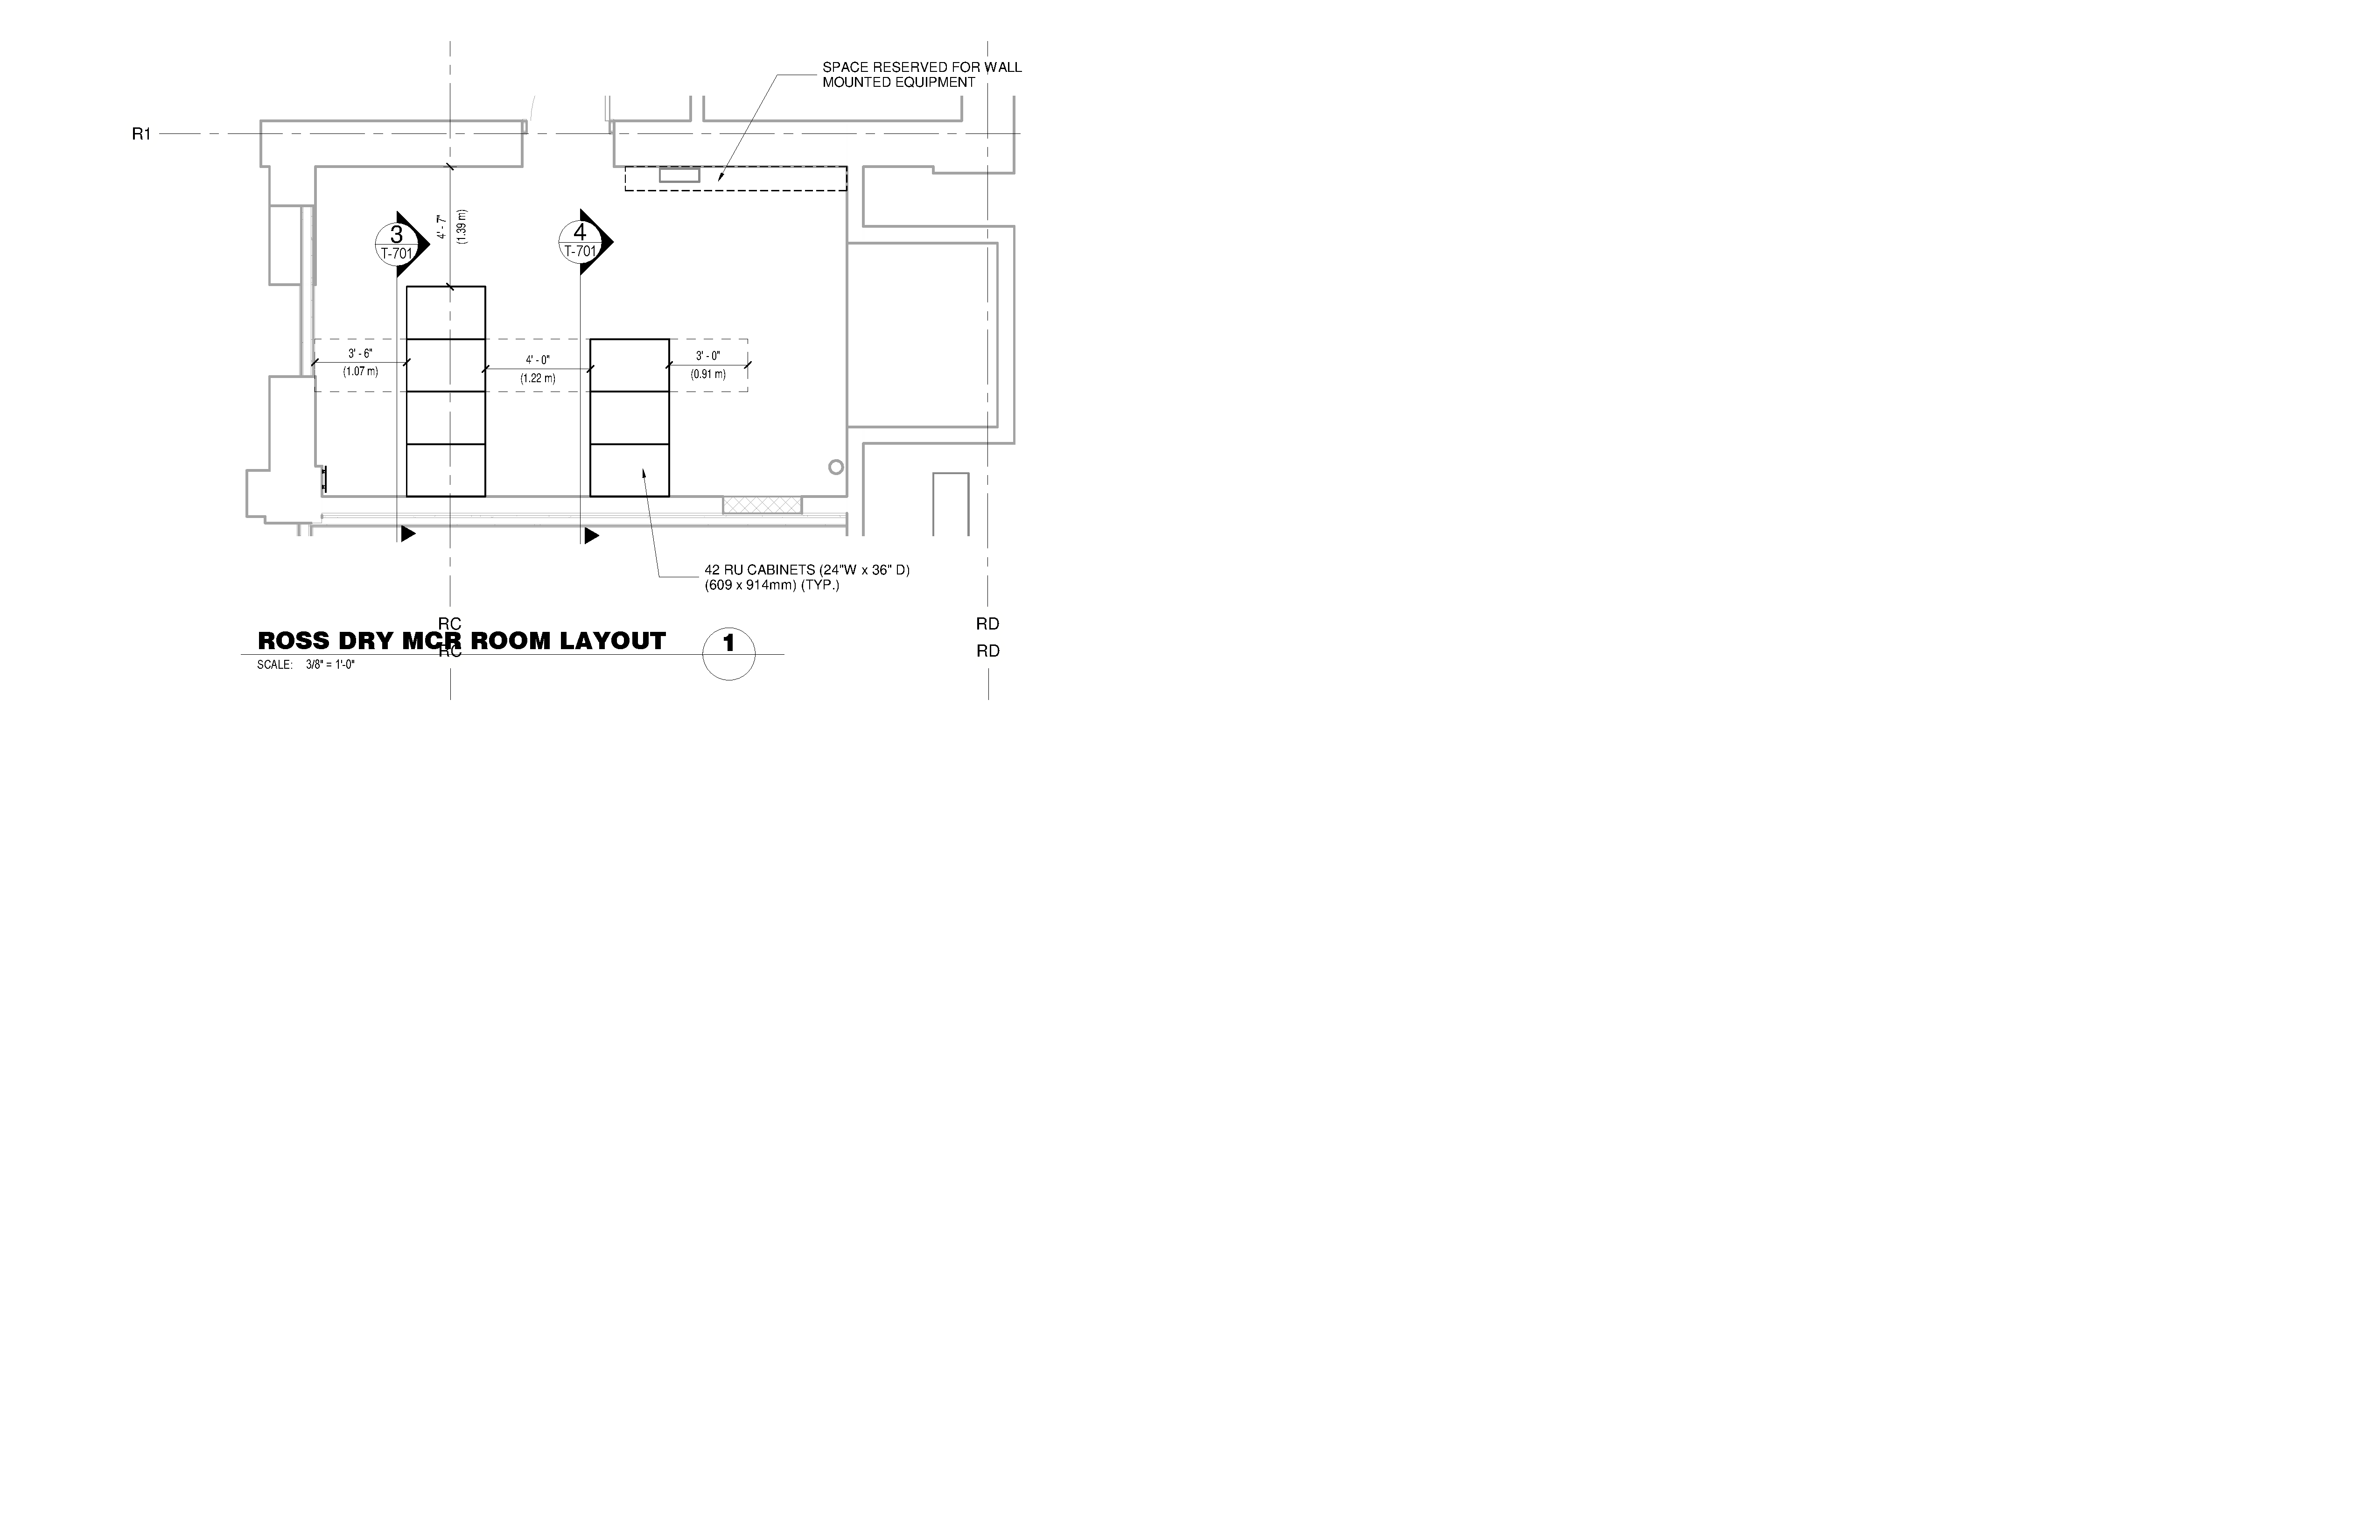
\includegraphics[width=0.85\textwidth]{Surface_Network_Fiber_Optic_Distribution_Room}
\end{dunefigure}


\section{\dword{dune} Detector Safety System}
\label{sec:fdsp-coord-det-safety}


The \dword{ddss} functions to protect experimental equipment.  The
system must detect abnormal and potentially harmful operating
conditions.  It must recognize when conditions are not within the
bounds of normal operating parameters and automatically take
pre-defined protective actions.


The detector safety system must communicate to the \surf \dword{firus}
and the \dword{dune} slow controls system, which monitors detector
status.  Working together through communication links, these three
systems can monitor the status of the experiment, protect equipment
and provide life safety. Figure~\ref{fig:dune-DDSS} indicates how
these systems interact.
\begin{dunefigure}[\dword{ddss}]{fig:dune-DDSS}
  {\dword{ddss} block diagram.}
  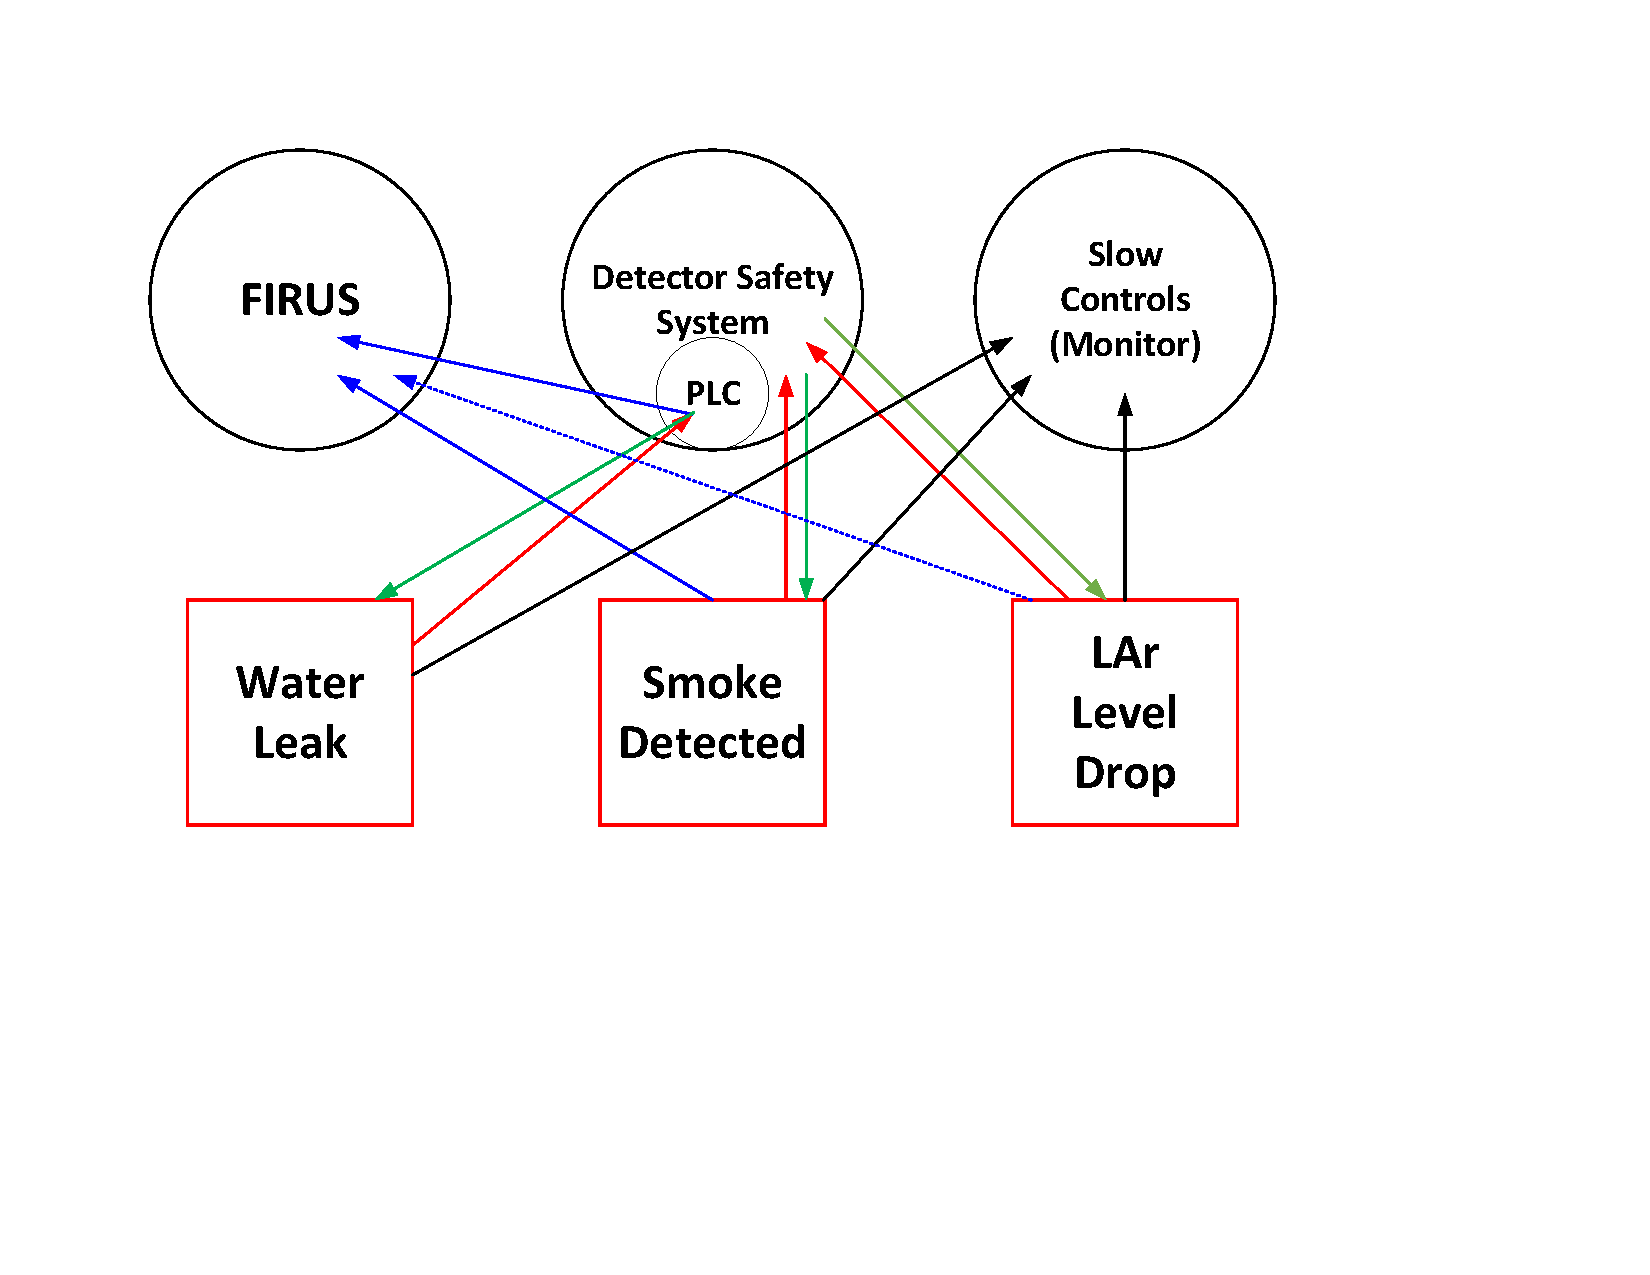
\includegraphics[width=0.85\textwidth]{DSS_Block_Diagram.pdf}
\end{dunefigure}


The \dword{ddss} will be implemented through hardware interlocks and a
\dword{plc}.  Listed below are some of \dword{dune} experimental
conditions that require intervention by the \dword{ddss}:
\begin{enumerate}
 \item A drop in the \dword{lar} level.  This condition requires a hardware
   interlock on the liquid level.  If the level drops below a
   pre-determined level, the drift high voltage must be automatically 
   shut off to prevent equipment damage.  Slow controls would be
   alerted through normal monitoring.
 \item Smoke or a temperature/humidity increase above normal operating
   levels. This is detected inside a rack or near an instrumented
   feedthrough.  If either of these conditions is detected, local
   power must be switched off. If smoke is detected, a
   dry contact will alert \dword{firus}.
 \item A water leak detected near energized equipment in the \dword{daq}
   underground data processing room.  Water leak detectors 
   report to the \dword{ddss} \dword{plc} and a decision will be made to either
   issue an alert or immediately shut power down to the room depending
   on the alert level.  This condition would also be reported
   to \dword{firus}.
\end{enumerate}
